% Finite-Elemente (ZHAW) — Beamer-Template
% (Passe Titel/Dozent/Datum nach Bedarf an.)

\documentclass[aspectratio=169,professionalfonts]{beamer}

% --- Sprache/Encoding ---
\usepackage[ngerman]{babel}
\usepackage[T1]{fontenc}
\usepackage[utf8]{inputenc}
\usepackage{lmodern}

% --- Mathe & Grafik ---
\usepackage{amsmath,amssymb,bm}
\usepackage{mathtools}
\usepackage{graphicx}
\usepackage{tikz}
\usetikzlibrary{arrows.meta,positioning,calc,decorations.pathmorphing,matrix,fit,backgrounds}

% --- Tabellen/Listen ---
\usepackage{booktabs}
\usepackage{multicol}

% --- Theme/Look ---
\usetheme{Madrid}
\usecolortheme{default}
\setbeamertemplate{navigation symbols}{}

% Fußzeile: Foliennummern
\setbeamertemplate{footline}{%
  \leavevmode%
  \hbox{%
  \begin{beamercolorbox}[wd=.8\paperwidth,ht=2.5ex,dp=1.1ex,left]{author in head/foot}\hspace{1em}\insertshortauthor\hspace{1em}--\hspace{1em}\insertshorttitle\end{beamercolorbox}%
  \begin{beamercolorbox}[wd=.2\paperwidth,ht=2.5ex,dp=1.1ex,right]{date in head/foot}\insertframenumber{} / \inserttotalframenumber\hspace{1em}\end{beamercolorbox}}%
  \vskip0pt%
}

% --- Metadaten ---
\title[FEM]{Finite Elemente Methode}
\subtitle{Vorlesung}
\author[ZHAW]{Sebastian Domaschke}
\institute[ZHAW]{Zürcher Hochschule für Angewandte Wissenschaften (ZHAW)}
\date{Frühlingssemester 2026}
\titlegraphic{
\includegraphics[height=1.2cm]{../Grafiken/logo.pdf}}

% --- Nützliche Makros ---
\newcommand{\R}{\mathbb{R}}
\newcommand{\dd}{\,\mathrm{d}}
\newcommand{\grad}{\nabla}
\newcommand{\K}{\underline{\underline{K}}}
\newcommand{\fvec}{\mathbf{f}}
\newcommand{\uvec}{\mathbf{u}}
\newcommand{\mat}[1]{\underline{\underline{#1}}}

% --- Fachwerk-Skizze (TikZ, skalierbar) ---
% Verwendung: \FachwerkSkizze  oder  \resizebox{\linewidth}{!}{\FachwerkSkizze}
\newcommand{\FachwerkSkizze}{%
\begin{tikzpicture}[scale=0.99, every node/.style={font=\small},
    disp/.style={draw=green!70!black, very thick, -{Latex[length=3mm]}, green!70!black},
    load/.style={draw=red!80!black, very thick, -{Latex[length=3mm]}, red!80!black},
    member/.style={line width=1.2pt, black},
    joint/.style={circle, fill=black, inner sep=2.2pt},
    elbox/.style={draw, rectangle, inner sep=2pt, fill=white}
  ]
    % Knoten
    \coordinate (n1) at (0,0);
    \coordinate (n2) at (4,0);
    \coordinate (n3) at (4,3);
    \coordinate (n4) at (8,3);

    % Stäbe (Elemente)
    \draw[member] (n1) -- (n2); % e1
    \draw[member] (n1) -- (n3); % e2
    \draw[member] (n2) -- (n3); % e3
    \draw[member] (n2) -- (n4); % e4
    \draw[member] (n3) -- (n4); % e5

    % Gelenke
    \node[joint] at (n1) {};
    \node[joint] at (n2) {};
    \node[joint] at (n3) {};
    \node[joint] at (n4) {};

    % Knotennummern
    \node[above left] at (n1) {$1$};
    \node[above left] at (n2) {$2$};
    \node[above left] at (n3) {$3$};
    \node[above left] at (n4) {$4$};

    % Elementnummern
    \node[elbox] at (2.0,-0.35) {$1$};
    \node[elbox] at (1.8,1.45) {$2$};
    \node[elbox] at (4.25,1.5) {$3$};
    \node[elbox] at (6.0,1.35) {$4$};
    \node[elbox] at (6.0,3.25) {$5$};

    % Lager
    \draw[line width=1pt] (n1) ++(-0.35,-0.35) -- ++(0.70,0) ;
    \draw[line width=1pt] (n1) ++(-0.35,-0.35) -- (n1);
    \draw[line width=1pt] (n1) ++(0.35,-0.35) -- (n1);
    \foreach \xx in {-0.40,-0.28,...,0.40} {\draw (n1) ++(\xx,-0.35) -- ++(0.12,-0.12);}

    % Loslager Knoten 2: Dreieck auf Gleitplatte (frei in x-Richtung)
    \draw[line width=1pt] (n2) ++(-0.35,-0.35) -- (n2);
    \draw[line width=1pt] (n2) ++(0.35,-0.35) -- (n2);
    \draw[line width=1pt] (n2) ++(-0.35,-0.35) -- ++(0.70,0);
    \draw[line width=1pt] (n2) ++(-0.45,-0.47) -- ++(0.90,0);
    \foreach \xx in {-0.40,-0.28,...,0.40} {\draw (n2) ++(\xx,-0.47) -- ++(0.12,-0.12);}

    % Verschiebungen (grün) + zugehörige Knotenkräfte (rot)
    \pgfmathsetmacro{\L}{0.75}

    % Knoten 1
    \draw[disp] (n1) -- ++(\L,0) node[midway, below right] {\color{green!70!black}$U_1$};
    \draw[disp] (n1) -- ++(0,\L) node[above, left] {\color{green!70!black}$U_2$};

    % Knoten 2
    \draw[disp] (n2) -- ++(\L,0) node[midway, below right] {\color{green!70!black}$U_3$};
    \draw[disp] (n2) -- ++(0,\L) node[above, left] {\color{green!70!black}$U_4$};

    % Knoten 3
    \draw[disp] (n3) -- ++(\L,0) node[midway, above] {\color{green!70!black}$U_5$};
    \draw[disp] (n3) -- ++(0,\L) node[above, left] {\color{green!70!black}$U_6$};

    % Knoten 4
    \draw[disp] (n4) -- ++(\L,0) node[midway, above] {\color{green!70!black}$U_7$};
    \draw[disp] (n4) -- ++(0,\L) node[above, left] {\color{green!70!black}$U_8$};

    % Last (rot)
    \draw[load] (n4) -- ++(0,-1.4) node[right] {$F$};

    % Koordinatensystem
    \draw[->,thick] (6.8,0.1) -- ++(1.0,0) node[right] {$X$};
    \draw[->,thick] (6.8,0.1) -- ++(0,1.0) node[above] {$Y$};
  \end{tikzpicture}%
}

\begin{document}

% Titelfolie
\begin{frame}
  \titlepage
\end{frame}



\begin{frame}{Übergeordnetes Lernziel 2}
  \centering
  \begin{minipage}{0.9\linewidth}
    \centering
    {\LARGE  Herleitung / Erklärung FEM\\[0.6em]}
    {\Large bestehend aus 1D-Elementen (Federn, Stäben, Balken)\\[0.4em]}
    {\Large mittels \textbf{Matrixsteifigkeitsmethode}}
  \end{minipage}
\end{frame}

\begin{frame}{Lernziele Vorlesung}
  \small
  Sie können
  \begin{enumerate}
    \item die Elementsteifigkeitsmatrizen zur Struktursteifigkeitsmatrix zusammenbauen.
    \item das Gleichungssystem $\mathbf{F}=\underline{\underline{K}}\mathbf{U}$ mit den Randbedingungen so umgruppieren, dass es lösbar wird.
    \item das Gleichungssystem lösen, d.\,h. die unbekannten Verschiebungen $\mathbf{U}_F$ und Zwangskräfte $\mathbf{F}_U$ berechnen.
    \item in der Nachlaufrechnung ausgehend vom Verschiebungsvektor $\mathbf{U}$ die Dehnungen $\varepsilon_e$ und Spannungen $\sigma_e$ der Elemente berechnen.
    \item Einführung Balkenelement (Ausblick)
  \end{enumerate}
\end{frame}



\begin{frame}{Tafelbild Befüllung Struktursteifigkeitsmatrix}
  \centering
\end{frame}
\begin{frame}{Fachwerk: Freiheitsgrade und Knotenkräfte}
  \centering
  \FachwerkSkizze
\end{frame}
\begin{frame}{Wiederholung}
  \centering
  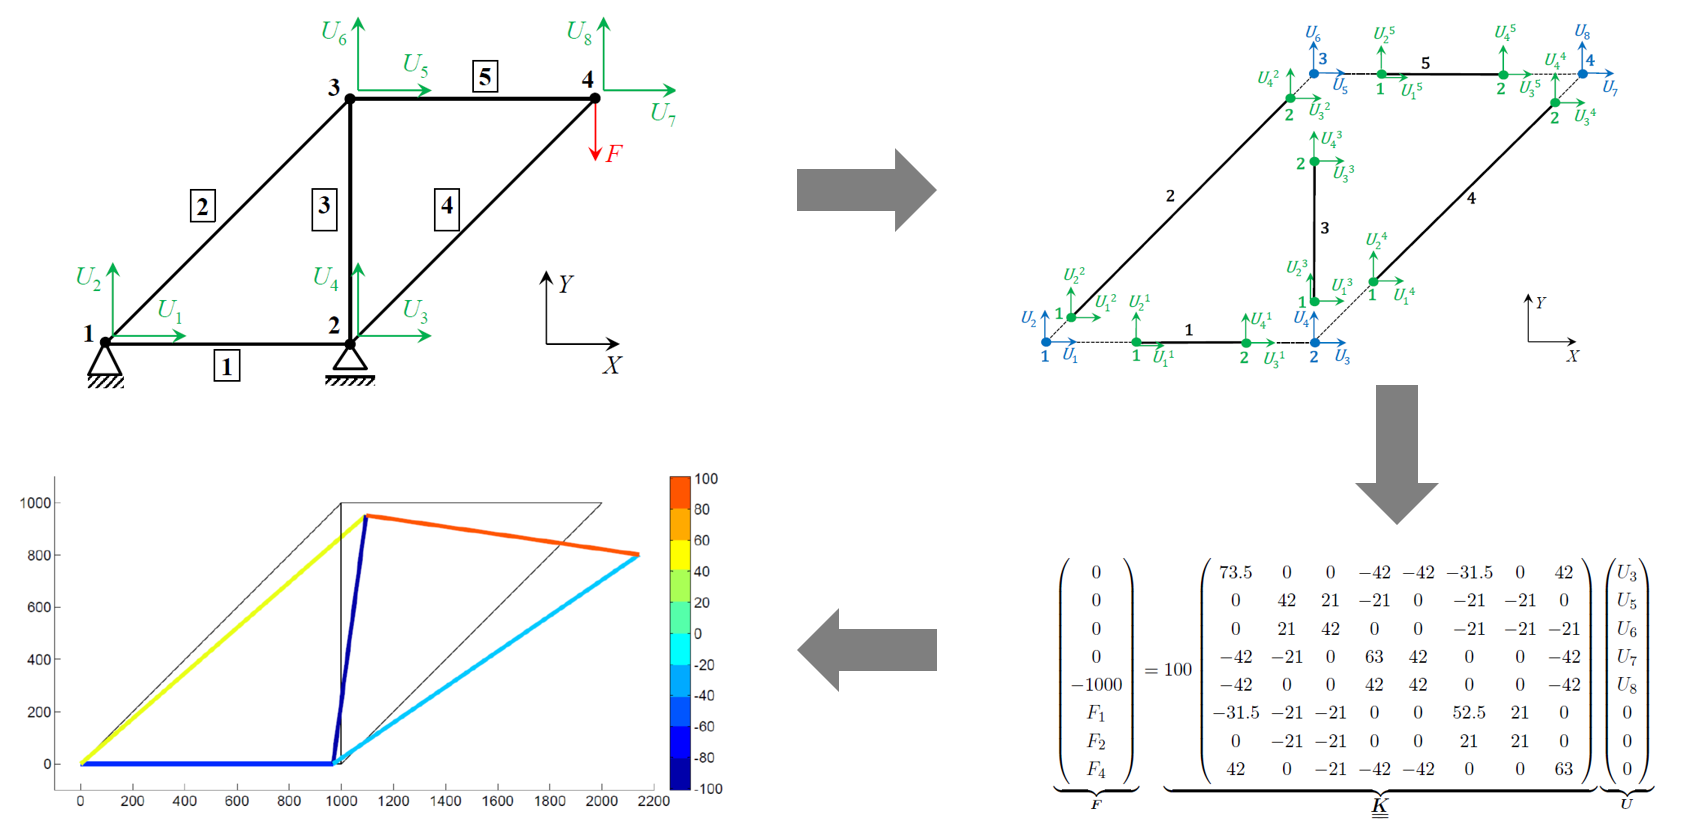
\includegraphics[width=\textwidth]{../Grafiken/Wiederholung0.png}
\end{frame}

\begin{frame}{Wiederholung}
  \centering
  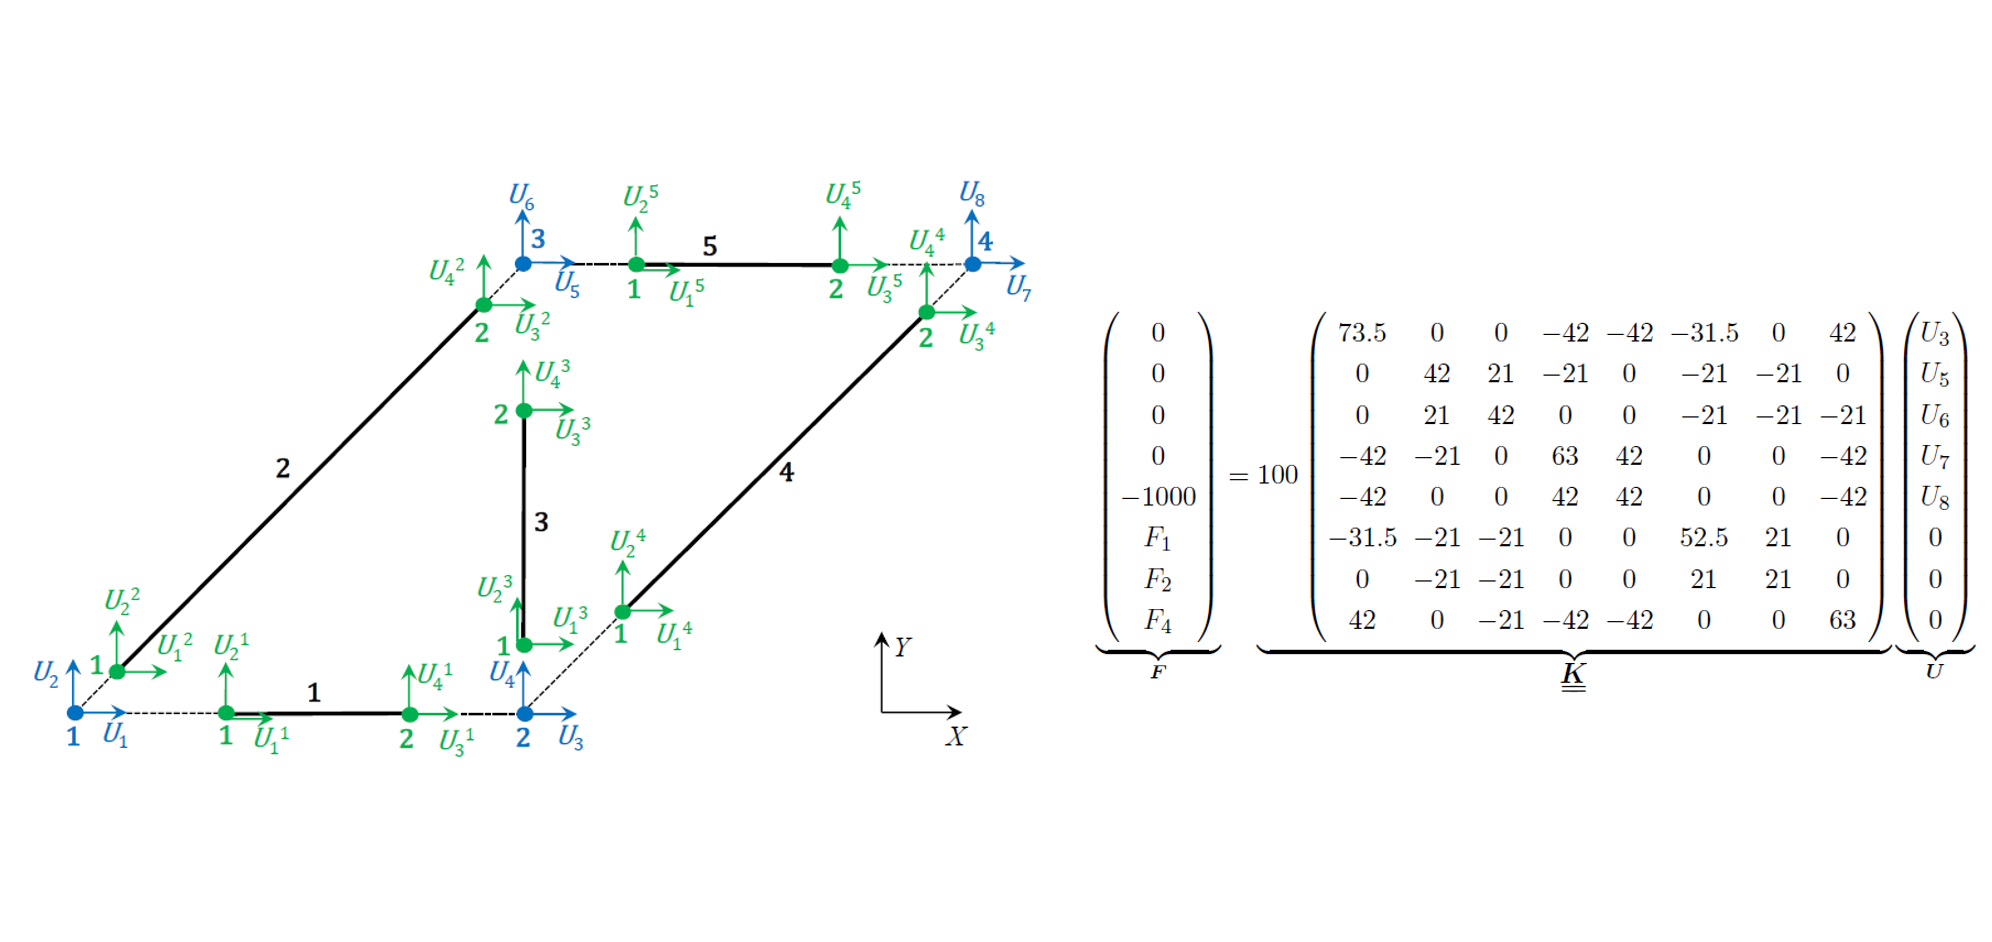
\includegraphics[width=\textwidth]{../Grafiken/Wiederholung1.png}
\end{frame}


\begin{frame}{Wiederholung}
  \centering
  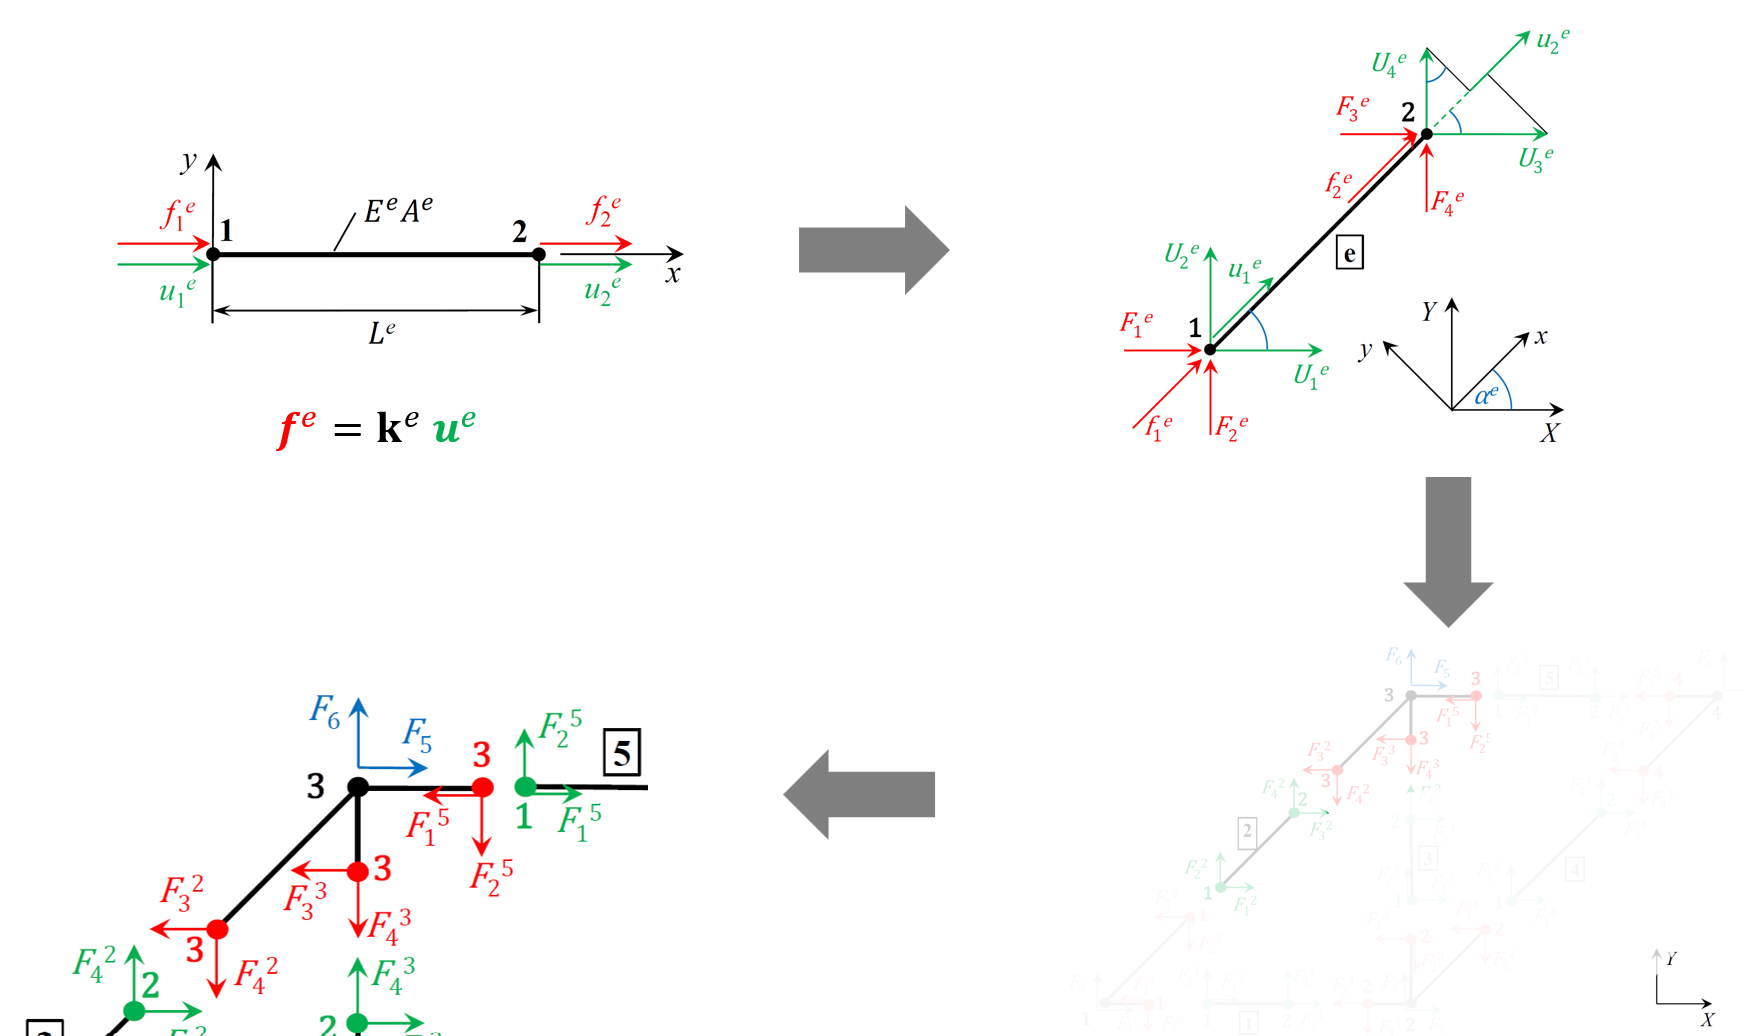
\includegraphics[height=\textheight]{../Grafiken/Wiederholung2.png}
\end{frame}

\begin{frame}{Wiederholung}
  \centering
  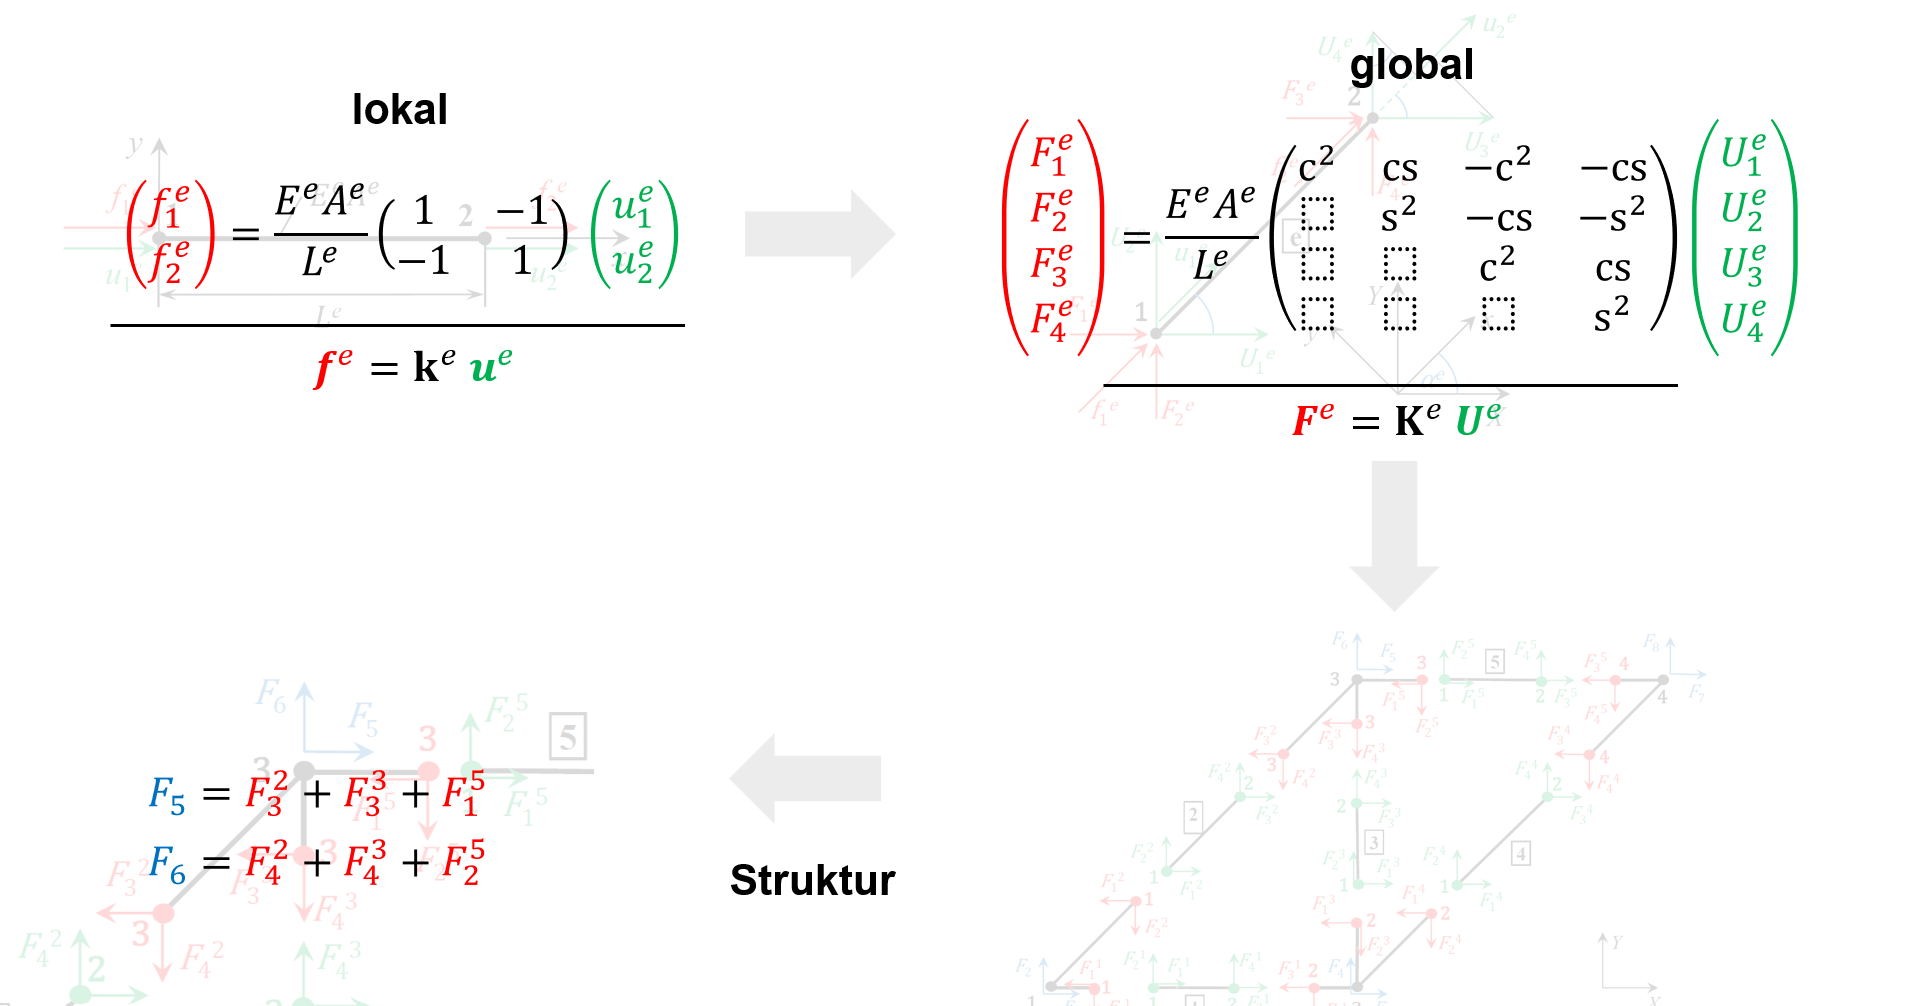
\includegraphics[height=\textheight]{../Grafiken/Wiederholung3.png}
\end{frame}

\begin{frame}{Fachwerk: Gleichungssystem aufstellen und Randbedingungen einfügen}
\scriptsize
\textbf{Einpflegen der Randbedingungen} -- Um das lineare Gleichungssystem lösbar zu machen, müssen die Randbedingungen eingepflegt werden. Ziel: $\underline{\underline{K}}$ ist nicht mehr singulär.

\vspace{0.5em}   
\begin{tabular}{@{}ll@{\quad}ll@{}}
  \textbf{Verschiebungs-/geom.\ RB:} & $U_1=U_2=U_4=0$ &
  \textbf{Unbekannte Reaktionskräfte:} & $F_1,\,F_2,\,F_4$ \\[0.4em]
  \textbf{Kraft-/natürliche RB:} & $F_3=F_5=F_6=F_7=0,\; F_8=-F$ &
  \textbf{Unbekannte Verschiebungen:} & $U_3,\,U_5,\,U_6,\,U_7,\,U_8$ \\
\end{tabular}
\vspace{2.5em}
\smallskip
\begin{columns}[T,onlytextwidth]
  \begin{column}{0.34\textwidth}
    \resizebox{\linewidth}{!}{\FachwerkSkizze}
  \end{column}
  \begin{column}{0.74\textwidth}
    \centering
    \begin{tikzpicture}[
      ampersand replacement=\&,
      every node/.style={font=\scriptsize, anchor=center},
      knownF/.style={fill=orange!22, rounded corners=1pt, opacity=0.65},
      knownU/.style={fill=green!22,  rounded corners=1pt, opacity=0.65}
    ]
  \matrix (F) [matrix of math nodes, nodes in empty cells,
    row sep=0.45ex, column sep=0.6ex,
    nodes={inner sep=1.0pt, minimum height=1.45ex, minimum width=1.6em},
    left delimiter=(, right delimiter=)
  ]{
    F_1 \\
    F_2 \\
    0 \\
    F_4 \\
    0 \\
    0 \\
    0 \\
    {-F} \\
  };

  \node (eq1) [right=0.8em of F] {$=$};

  \matrix (K) [right=0.8em of eq1, matrix of math nodes, nodes in empty cells,
    row sep=0.45ex, column sep=0.55ex,
    nodes={inner sep=1.0pt, minimum height=1.45ex, minimum width=1.75em},
    left delimiter=(, right delimiter=)
  ]{
    K_{11} \& K_{12} \& K_{13} \& K_{14} \& K_{15} \& K_{16} \& K_{17} \& K_{18} \\
    K_{21} \& K_{22} \& K_{23} \& K_{24} \& K_{25} \& K_{26} \& K_{27} \& K_{28} \\
    K_{31} \& K_{32} \& K_{33} \& K_{34} \& K_{35} \& K_{36} \& K_{37} \& K_{38} \\
    K_{41} \& K_{42} \& K_{43} \& K_{44} \& K_{45} \& K_{46} \& K_{47} \& K_{48} \\
    K_{51} \& K_{52} \& K_{53} \& K_{54} \& K_{55} \& K_{56} \& K_{57} \& K_{58} \\
    K_{61} \& K_{62} \& K_{63} \& K_{64} \& K_{65} \& K_{66} \& K_{67} \& K_{68} \\
    K_{71} \& K_{72} \& K_{73} \& K_{74} \& K_{75} \& K_{76} \& K_{77} \& K_{78} \\
    K_{81} \& K_{82} \& K_{83} \& K_{84} \& K_{85} \& K_{86} \& K_{87} \& K_{88} \\
  };

  \matrix (U) [right=2.0em of K, matrix of math nodes, nodes in empty cells,
    row sep=0.45ex, column sep=0.6ex,
    nodes={inner sep=1.0pt, minimum height=1.45ex, minimum width=1.6em},
    left delimiter=(, right delimiter=)
  ]{
    0 \\
    0 \\
    U_3 \\
    0 \\
    U_5 \\
    U_6 \\
    U_7 \\
    U_8 \\
  };

  \begin{pgfonlayer}{background}
    \foreach \r in {3,5,6,7,8} {\node[knownF, fit=(F-\r-1), inner sep=0pt] {};}
    \foreach \r in {1,2,4}     {\node[knownU, fit=(U-\r-1), inner sep=0pt] {};}
  \end{pgfonlayer}
\end{tikzpicture}

\vspace{0.2em}
\centering
$\mathbf{F}=\underline{\underline{K}}\mathbf{U}$
  \end{column}
\end{columns}
\end{frame}

\begin{frame}{Lösung Gleichungssystem}
\scriptsize

\begin{columns}[T,onlytextwidth]
  \begin{column}{0.34\textwidth}
    % Bild hier einfügen/ersetzen
    \resizebox{\linewidth}{!}{\FachwerkSkizze}

    \vfill
    \onslide<2->{%
      \text{Löse Gleichungssystem durch:}
      {\scriptsize
      \begin{align*}
        \fcolorbox{magenta!80!black}{white}{$\mathbf{F}_F$}
        &=
        \fcolorbox{orange!80!black}{white}{$\underline{\underline{K}}_{FF}$}
        \fcolorbox{cyan!70!black}{white}{$\mathbf{U}_F$}
        +
        \fcolorbox{blue!70!black}{white}{$\underline{\underline{K}}_{FU}$}
        \fcolorbox{purple!70!black}{white}{$\mathbf{U}_U$}
        \\
        \fcolorbox{teal!80!black}{white}{$\mathbf{F}_U$}
        &=
        \fcolorbox{red!80!black}{white}{$\underline{\underline{K}}_{UF}$}
        \fcolorbox{cyan!70!black}{white}{$\mathbf{U}_F$}
        +
        \fcolorbox{green!60!black}{white}{$\underline{\underline{K}}_{UU}$}
        \fcolorbox{purple!70!black}{white}{$\mathbf{U}_U$}
        \\
        \mathbf{U}_F &= \underline{\underline{K}}_{FF}^{-1}\bigl(\mathbf{F}_F - \underline{\underline{K}}_{FU}\mathbf{U}_U\bigr)\\
        \mathbf{F}_U &= \underline{\underline{K}}_{UF}\mathbf{U}_F + \underline{\underline{K}}_{UU}\mathbf{U}_U
      \end{align*}

      {\tiny Hinweis: Bei homogenen Randbedingungen (wie in diesem Beispiel) gilt $\mathbf{U}_U=\mathbf{0}$.}
      }%
    }
  \end{column}
  \begin{column}{0.74\textwidth}
    \centering
    \begin{tikzpicture}[
      ampersand replacement=\&,
      every node/.style={font=\scriptsize, anchor=center},
      knownF/.style={fill=orange!22, rounded corners=1pt, opacity=0.65},
      knownU/.style={fill=green!22,  rounded corners=1pt, opacity=0.65}
    ]
  \matrix (F) [matrix of math nodes, nodes in empty cells,
    row sep=0.45ex, column sep=0.6ex,
    nodes={inner sep=1.0pt, minimum height=1.45ex, minimum width=1.6em},
    left delimiter=(, right delimiter=)
  ]{
    F_1 \\
    F_2 \\
    0 \\
    F_4 \\
    0 \\
    0 \\
    0 \\
    {-F} \\
  };

  \node (eq1) [right=0.8em of F] {$=$};

  \matrix (K) [right=0.8em of eq1, matrix of math nodes, nodes in empty cells,
    row sep=0.45ex, column sep=0.55ex,
    nodes={inner sep=1.0pt, minimum height=1.45ex, minimum width=1.75em},
    left delimiter=(, right delimiter=)
  ]{
    K_{11} \& K_{12} \& K_{13} \& K_{14} \& K_{15} \& K_{16} \& K_{17} \& K_{18} \\
    K_{21} \& K_{22} \& K_{23} \& K_{24} \& K_{25} \& K_{26} \& K_{27} \& K_{28} \\
    K_{31} \& K_{32} \& K_{33} \& K_{34} \& K_{35} \& K_{36} \& K_{37} \& K_{38} \\
    K_{41} \& K_{42} \& K_{43} \& K_{44} \& K_{45} \& K_{46} \& K_{47} \& K_{48} \\
    K_{51} \& K_{52} \& K_{53} \& K_{54} \& K_{55} \& K_{56} \& K_{57} \& K_{58} \\
    K_{61} \& K_{62} \& K_{63} \& K_{64} \& K_{65} \& K_{66} \& K_{67} \& K_{68} \\
    K_{71} \& K_{72} \& K_{73} \& K_{74} \& K_{75} \& K_{76} \& K_{77} \& K_{78} \\
    K_{81} \& K_{82} \& K_{83} \& K_{84} \& K_{85} \& K_{86} \& K_{87} \& K_{88} \\
  };

  \matrix (U) [right=2.0em of K, matrix of math nodes, nodes in empty cells,
    row sep=0.45ex, column sep=0.6ex,
    nodes={inner sep=1.0pt, minimum height=1.45ex, minimum width=1.6em},
    left delimiter=(, right delimiter=)
  ]{
    0 \\
    0 \\
    U_3 \\
    0 \\
    U_5 \\
    U_6 \\
    U_7 \\
    U_8 \\
  };

  \begin{pgfonlayer}{background}
    \foreach \r in {3,5,6,7,8} {\node[knownF, fit=(F-\r-1), inner sep=0pt] {};}
    \foreach \r in {1,2,4}     {\node[knownU, fit=(U-\r-1), inner sep=0pt] {};}
  \end{pgfonlayer}
\end{tikzpicture}

\vspace{0.2em}

\centering
$\mathbf{F}=\underline{\underline{K}}\mathbf{U}$

\vspace{0.05em}

\centering
\begin{tikzpicture}[
  ampersand replacement=\&,
  every node/.style={font=\scriptsize, anchor=center},
  knownF/.style={fill=orange!22, rounded corners=1pt, opacity=0.65},
  knownU/.style={fill=green!22,  rounded corners=1pt, opacity=0.65}
]
  % --- Permutierte / blockierte Darstellung ---
  \matrix (Fp) [matrix of math nodes, nodes in empty cells,
    row sep=0.22ex, column sep=0.6ex,
    nodes={inner sep=0.8pt, minimum height=1.2ex, minimum width=1.6em},
    left delimiter=(, right delimiter=)
  ]{
    0 \\
    0 \\
    0 \\
    0 \\
    {-F} \\
    F_1 \\
    F_2 \\
    F_4 \\
  };

  \node (eq2) [right=0.8em of Fp] {$=$};

  \matrix (Kp) [right=1.0em of eq2, matrix of math nodes, nodes in empty cells,
    row sep=0.22ex, column sep=0.45ex,
    nodes={inner sep=0.8pt, minimum height=1.2ex, minimum width=1.6em},
    left delimiter=(, right delimiter=)
  ]{
    K_{33} \& K_{35} \& K_{36} \& K_{37} \& K_{38} \& K_{31} \& K_{32} \& K_{34} \\
    K_{53} \& K_{55} \& K_{56} \& K_{57} \& K_{58} \& K_{51} \& K_{52} \& K_{54} \\
    K_{63} \& K_{65} \& K_{66} \& K_{67} \& K_{68} \& K_{61} \& K_{62} \& K_{64} \\
    K_{73} \& K_{75} \& K_{76} \& K_{77} \& K_{78} \& K_{71} \& K_{72} \& K_{74} \\
    K_{83} \& K_{85} \& K_{86} \& K_{87} \& K_{88} \& K_{81} \& K_{82} \& K_{84} \\
    K_{13} \& K_{15} \& K_{16} \& K_{17} \& K_{18} \& K_{11} \& K_{12} \& K_{14} \\
    K_{23} \& K_{25} \& K_{26} \& K_{27} \& K_{28} \& K_{21} \& K_{22} \& K_{24} \\
    K_{43} \& K_{45} \& K_{46} \& K_{47} \& K_{48} \& K_{41} \& K_{42} \& K_{44} \\
  };

  % Blockrahmen
  \draw[orange!80!black, line width=0.8pt] (Kp-1-1.north west) rectangle (Kp-5-5.south east);
  \draw[blue!70!black,   line width=0.8pt] (Kp-1-6.north west) rectangle (Kp-5-8.south east);
  \draw[red!80!black,    line width=0.8pt] (Kp-6-1.north west) rectangle (Kp-8-5.south east);
  \draw[green!60!black,  line width=0.8pt] (Kp-6-6.north west) rectangle (Kp-8-8.south east);

  \matrix (Up) [right=2.0em of Kp, matrix of math nodes, nodes in empty cells,
    row sep=0.22ex, column sep=0.6ex,
    nodes={inner sep=0.8pt, minimum height=1.2ex, minimum width=1.6em},
    left delimiter=(, right delimiter=)
  ]{
    U_3 \\
    U_5 \\
    U_6 \\
    U_7 \\
    U_8 \\
    0 \\
    0 \\
    0 \\
  };

  \begin{pgfonlayer}{background}
    % Kräfte: F_F (magenta), F_U (teal)
    \draw[magenta!80!black, line width=0.8pt] (Fp-1-1.north west) rectangle (Fp-5-1.south east);
    \draw[teal!80!black,    line width=0.8pt] (Fp-6-1.north west) rectangle (Fp-8-1.south east);

    % Verschiebungen: U_F (cyan), U_U (violett)
    \draw[cyan!70!black, line width=0.8pt] (Up-1-1.north west) rectangle (Up-5-1.south east);
    \draw[purple!70!black, line width=0.8pt] (Up-6-1.north west) rectangle (Up-8-1.south east);
  \end{pgfonlayer}
\end{tikzpicture}

\vspace{0.1em}

$\displaystyle \begin{pmatrix}\mathbf{F}_F\\ \mathbf{F}_U\end{pmatrix}=
\begin{pmatrix}\underline{\underline{K}}_{FF} & \underline{\underline{K}}_{FU}\\ \underline{\underline{K}}_{UF} & \underline{\underline{K}}_{UU}\end{pmatrix}
\begin{pmatrix}\mathbf{U}_F\\ \mathbf{U}_U\end{pmatrix}$

  \end{column}
\end{columns}
\end{frame}

\begin{frame}{Formalisierung Zusammenbau Struktursteifigkeitsmatrix}
  \small
  \textbf{Koinzidenztabelle}

  \vspace{0.5em}
  \centering
  \scriptsize
  \begin{tabular}{c|*{5}{c|}}
    \toprule
    Elementnummer $e$ & 1 & 2 & 3 & 4 & 5 \\
    \midrule
    \begin{tabular}{@{}c@{}}
      Elementverschiebung $U_j^{e}$\\
      wird abgebildet auf\\
      Gesamtverschiebung $U_l$
    \end{tabular}
    &
    $\begin{matrix}
      1 & 2 & 3 & 4\\[-0.2em]
      \downarrow & \downarrow & \downarrow & \downarrow\\[-0.2em]
      1 & 2 & 3 & 4
    \end{matrix}$
    &
    $\begin{matrix}
      1 & 2 & 3 & 4\\[-0.2em]
      \downarrow & \downarrow & \downarrow & \downarrow\\[-0.2em]
      1 & 2 & 5 & 6
    \end{matrix}$
    &
    $\begin{matrix}
      1 & 2 & 3 & 4\\[-0.2em]
      \downarrow & \downarrow & \downarrow & \downarrow\\[-0.2em]
      3 & 4 & 5 & 6
    \end{matrix}$
    &
    $\begin{matrix}
      1 & 2 & 3 & 4\\[-0.2em]
      \downarrow & \downarrow & \downarrow & \downarrow\\[-0.2em]
      3 & 4 & 7 & 8
    \end{matrix}$
    &
    $\begin{matrix}
      1 & 2 & 3 & 4\\[-0.2em]
      \downarrow & \downarrow & \downarrow & \downarrow\\[-0.2em]
      5 & 6 & 7 & 8
    \end{matrix}$
    \\
    \bottomrule
  \end{tabular}

  \vspace{0.4em}
  \raggedright
  \textbf{Koinzidenzmatrix}\\[0.25em]
  Aus der Koinzidenztabelle kann die Verbindung von Elementverschiebungen $\mathbf{u}^{e}$ (global)
  und Knotenverschiebungen der Struktur $\mathbf{U}$ hergestellt werden
  $\Rightarrow$ hier am Beispiel des Elements $2$:
  \vspace{-1.5em}
  \centering
  \scriptsize
  \[
    \scalebox{0.9}{$
    \begin{pmatrix}
      U^{2}_{1} \\[0.2em]
      U^{2}_{2} \\[0.2em]
      U^{2}_{3} \\[0.2em]
      U^{2}_{4}
    \end{pmatrix}
    =
    \begin{pmatrix}
      1 & 0 & 0 & 0 & 0 & 0 & 0 & 0 \\
      0 & 1 & 0 & 0 & 0 & 0 & 0 & 0 \\
      0 & 0 & 0 & 0 & 1 & 0 & 0 & 0 \\
      0 & 0 & 0 & 0 & 0 & 1 & 0 & 0
    \end{pmatrix}
    \begin{pmatrix}
      U_{1} \\[0.2em]
      U_{2} \\[0.2em]
      U_{3} \\[0.2em]
      U_{4} \\[0.2em]
      U_{5} \\[0.2em]
      U_{6} \\[0.2em]
      U_{7} \\[0.2em]
      U_{8}
    \end{pmatrix}
    $}
  \]
\vspace{-1.5em}

\centering
\scriptsize
$\mathbf{U}^{2} = \underline{\underline{\hat{T}}}^{\,2}\,\mathbf{U}$ \\[0.4em]
\fbox{Allgemein: \quad $\mathbf{U}^{e} = \underline{\underline{\hat{T}}}^{\,e}\,\mathbf{U}$ \quad $\underline{\underline{\hat{T}}}^{\,e}$ Koinzidenzmatrix des Elementes $e$}
\end{frame}

\begin{frame}{Koinzidenzmatrix $\Rightarrow$ Knotengleichgewicht}
  \centering

  \vspace{0.6em}
  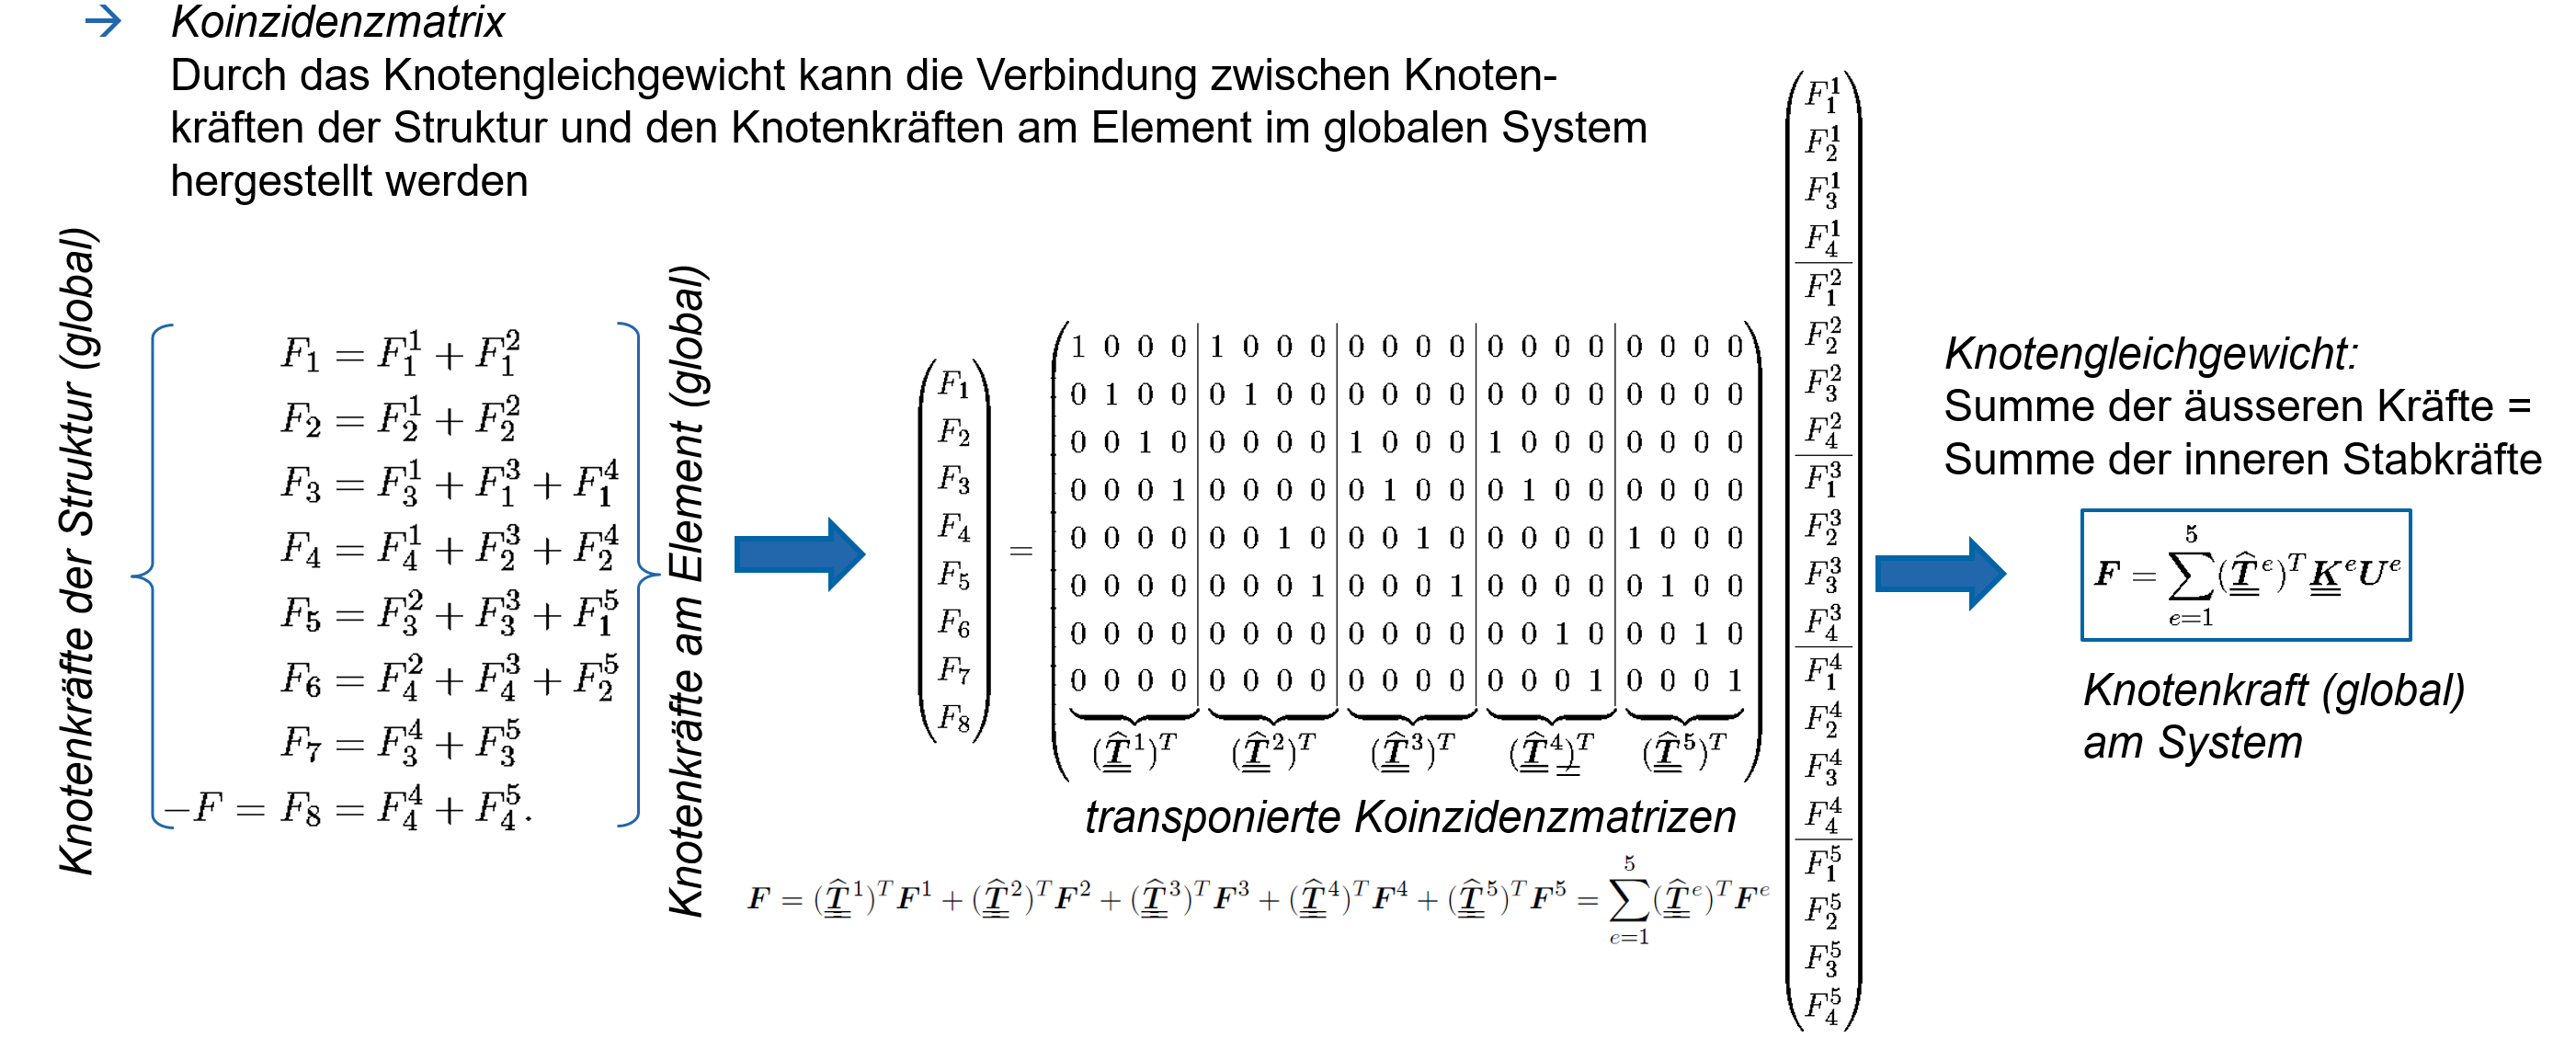
\includegraphics[width=\textwidth]{../Grafiken/koinzidenzmatrix_knotengleichgewicht.png}
\end{frame}

\begin{frame}{Formalisierung Zusammenbau Struktursteifigkeitsmatrix (II)}
\small

\textbf{Knotengleichgewicht:} Summe der äußeren Kräfte $=$ Summe der inneren Stabkräfte $\Rightarrow$ Knotenkraft am System:

\vspace{0.4em}
\centering
\fbox{%
  \begin{minipage}{0.72\linewidth}
    \centering\small
    $\mathbf{F} \;=\; \displaystyle\sum_{e=1}^{5} \left(\underline{\underline{\hat{T}}}^{\,e}\right)^{\!T}\,\mathbf{F}^{e}= \displaystyle\sum_{e=1}^{5} \left(\underline{\underline{\hat{T}}}^{\,e}\right)^{\!T}\,\underline{\underline{K}}^{e}\,\mathbf{U}^{e}$
  \end{minipage}
}

\vspace{0.6em}
\raggedright
Einsetzen von $\mathbf{U}^{e}=\underline{\underline{\hat{T}}}^{e}\mathbf{U}$ und Vergleich mit $\mathbf{F}=\underline{\underline{K}}\mathbf{U}$ $\Rightarrow$ \textit{Assembly} der Struktursteifigkeitsmatrix:

\vspace{0.4em}
\centering
\fbox{%
  \begin{minipage}{0.72\linewidth}
    \centering\small
    $\underline{\underline{K}} \;=\; \displaystyle\sum_{e=1}^{5} \left(\underline{\underline{\hat{T}}}^{\,e}\right)^{\!T}\,\underline{\underline{K}}^{e}\,\underline{\underline{\hat{T}}}^{\,e}$
  \end{minipage}
}

\end{frame}

\begin{frame}{Einführung eigener FEM Löser in Python auf Github}
  \centering
\end{frame}

\begin{frame}{1D-Stab-Element: Nachlaufrechnung}
  \centering
\begin{tikzpicture}[
    scale=0.58,
    every node/.style={font=\scriptsize},
    axis/.style={very thick, -{Latex[length=2.6mm]}},
    bar/.style={line width=1.8pt, black},
    joint/.style={circle, fill=blue!70, inner sep=2.2pt},
    uarr/.style={draw=green!70!black, very thick, -{Latex[length=2.6mm]}, green!70!black},
    farr/.style={draw=red!80!black,   very thick, -{Latex[length=2.6mm]}, red!80!black},
    dim/.style={thin, {Latex[length=2.3mm]}-{Latex[length=2.3mm]}}
  ]
    % Knotenkoordinaten
    \coordinate (n1) at (0,0);
    \coordinate (n2) at (8,0);

    % Stab
    \draw[bar] (n1) -- (n2);

    % Knotenpunkte
    \node[joint] at (n1) {};
    \node[joint] at (n2) {};

    % Knotennummern
    \node[blue!70!black, above right] at (n1) {\Large 1};
    \node[blue!70!black, above left] at (n2) {\Large 2};

    % Achsen (links y, rechts x) – mit Abstand zu den Knoten
    \draw[axis] ($(n1)+(0,0.15)$) -- ++(0,2.15) node[left] {$y$};
    \draw[axis] ($(n2)+(0.15,0)$) -- ++(2.45,0) node[below] {$x$};

    % Verschiebungen u^e (grün)
    \draw[uarr] (n1) ++(-1.6,-0.45) -- ++(1.6,0) node[midway, below] {$u_1^{e}$};
    \draw[uarr] (n2) ++(0.0,-0.45)  -- ++(1.6,0) node[midway, below] {$u_2^{e}$};

    % Knotenkräfte f^e (rot)
    \draw[farr] (n1) ++(-1.6,0.45) -- ++(1.6,0) node[midway, above] {$f_1^{e}$};
    \draw[farr] (n2) ++(0.0,0.45)  -- ++(1.6,0) node[midway, above] {$f_2^{e}$};

    % Material/Querschnitt
    \node[above] at ($(n1)!0.50!(n2)+(0,0.25)$) {$E^{e}A^{e}$};

    % L^e Dimension unten (mit Hilfslinien + Pfeile beidseitig)
    \draw[thin] (n1) -- ++(0,-1.0);
    \draw[thin] (n2) -- ++(0,-1.0);
    \draw[dim] ($(n1)+(0,-1.0)$) -- ($(n2)+(0,-1.0)$) node[midway, below] {$L^{e}$};
  \end{tikzpicture}

  \vspace{0.02em}

  % Formeln darunter
  \scriptsize
  \begin{align*}
    \text{Schritt 0: Globale Verschiebungen berechnet } \mathbf{U}&&
   \\
   \text{Schritt 1: lokale Elementverschiebungen berechnen}&&\mathbf{u}^{e} &= \mathbf{{T}}^{e}\mathbf{\hat{T}}^{e}\,\mathbf{U} = \bigl(u^{e}_{1}\; u^{e}_{2}\bigr)^{T}
   \\
    \text{Schritt 2: Dehnung im Stab berechnen}&&\mathbf{\varepsilon}^{e} &= \frac{\Delta L^{e}}{L^{e}} =\frac{u^{e}_{2}-u^{e}_{1}}{L^{e}} 
    \\
    \text{Schritt 3: Spannung im Stab berechnen}&&\mathbf{\sigma}^{e} &= E^{e}\varepsilon^{e}
  \end{align*}
\end{frame}

\begin{frame}{Tafelbild Balkenelement}
  \centering
\end{frame}
\begin{frame}{lokale Elementsteifigkeitsmatrix eines Biegebalkens (Beam)}
  \centering
  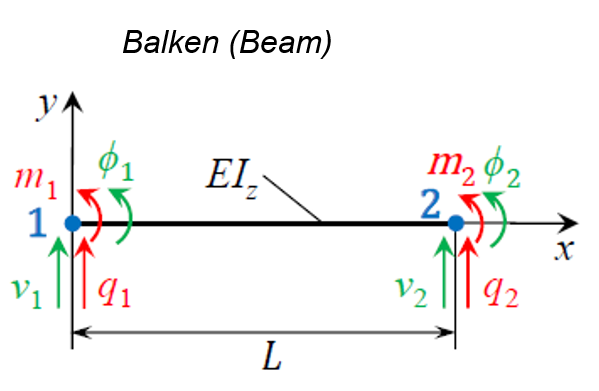
\includegraphics[width=0.32\linewidth]{../Grafiken/beam_skizze.png}

  \vspace{0.45em}
  \scriptsize
  \[
  \begin{pmatrix}
    q_1\\
    m_1\\
    q_2\\
    m_2
  \end{pmatrix}
  = E I_z
  \begin{pmatrix}
    \dfrac{12}{L^3} & \dfrac{6}{L^2}  & -\dfrac{12}{L^3} & \dfrac{6}{L^2} \\
    \dfrac{6}{L^2}  & \dfrac{4}{L}    & -\dfrac{6}{L^2}  & \dfrac{2}{L}   \\
    -\dfrac{12}{L^3} & -\dfrac{6}{L^2} & \dfrac{12}{L^3}  & -\dfrac{6}{L^2}\\
    \dfrac{6}{L^2}  & \dfrac{2}{L}    & -\dfrac{6}{L^2}  & \dfrac{4}{L}
  \end{pmatrix}
  \begin{pmatrix}
    v_1\\
    \phi_1\\
    v_2\\
    \phi_2
  \end{pmatrix}
  \]

  \vspace{0.3em}
  \[
    \mathbf{q}=\underline{\underline{k}}\,\mathbf{v}
  \]
\end{frame}





\begin{frame}{lokale Elementsteifigkeitsmatrix des Zug/Druck/Biegestabs}
  \centering
  \begin{columns}[T,onlytextwidth]
    \begin{column}{0.49\textwidth}
      \centering
      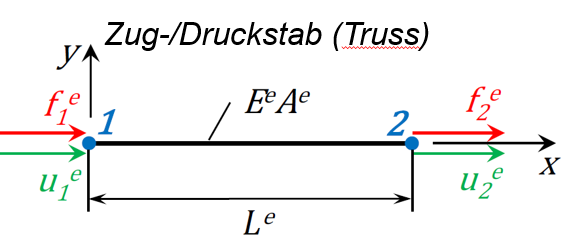
\includegraphics[width=0.70\linewidth]{../Grafiken/truss_skizze.png}
    \end{column}
    \begin{column}{0.49\textwidth}
      \centering
      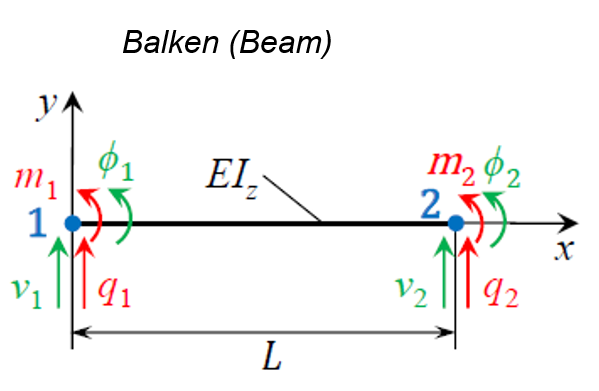
\includegraphics[width=0.60\linewidth]{../Grafiken/beam_skizze.png}
    \end{column}
  \end{columns}

  \vspace{0.25em}
  \scriptsize
  \[
  \begin{pmatrix}
    f_1\\
    q_1\\
    m_1\\
    f_2\\
    q_2\\
    m_2
  \end{pmatrix}
  = \frac{E}{L^3}
  \begin{pmatrix}
    AL^2 & 0 & 0 & -AL^2 & 0 & 0 \\
    0 & 12I_z & 6I_zL & 0 & -12I_z & 6I_zL \\
    0 & 6I_zL & 4I_zL^2 & 0 & -6I_zL & 2I_zL^2 \\
    -AL^2 & 0 & 0 & AL^2 & 0 & 0 \\
    0 & -12I_z & -6I_zL & 0 & 12I_z & -6I_zL \\
    0 & 6I_zL & 2I_zL^2 & 0 & -6I_zL & 4I_zL^2
  \end{pmatrix}
  \begin{pmatrix}
    u_1\\
    v_1\\
    \phi_1\\
    u_2\\
    v_2\\
    \phi_2
  \end{pmatrix}
  \]

  \vspace{0.2em}
  \[
    \mathbf{q}=\underline{\underline{k}}\,\mathbf{v}
  \]
\end{frame}



\begin{frame}{Transformation zur globalen Elementsteifigkeitsmatrix}
  \centering
  \small
  \[
    \underline{\underline{K}}^{e}=(\underline{\underline{T}}^{e})^{T}\,\underline{\underline{k}}^{e}\,\underline{\underline{T}}^{e}
  \]

  \vspace{0.25em}
  \tiny
  \[
  \resizebox{\linewidth}{!}{$
  \underline{\underline{K}}^{e}=
  \underbrace{\begin{pmatrix}
    c & -s & 0 & 0 & 0 & 0\\
    s &  c & 0 & 0 & 0 & 0\\
    0 &  0 & 1 & 0 & 0 & 0\\
    0 &  0 & 0 & c & -s & 0\\
    0 &  0 & 0 & s &  c & 0\\
    0 &  0 & 0 & 0 &  0 & 1
  \end{pmatrix}}_{(\underline{\underline{T}}^{e})^{T}}
  \underbrace{\begin{pmatrix}
    \dfrac{EA}{L} & 0 & 0 & -\dfrac{EA}{L} & 0 & 0\\
    0 & \dfrac{12EI_z}{L^3} & \dfrac{6EI_z}{L^2} & 0 & -\dfrac{12EI_z}{L^3} & \dfrac{6EI_z}{L^2}\\
    0 & \dfrac{6EI_z}{L^2} & \dfrac{4EI_z}{L} & 0 & -\dfrac{6EI_z}{L^2} & \dfrac{2EI_z}{L}\\
    -\dfrac{EA}{L} & 0 & 0 & \dfrac{EA}{L} & 0 & 0\\
    0 & -\dfrac{12EI_z}{L^3} & -\dfrac{6EI_z}{L^2} & 0 & \dfrac{12EI_z}{L^3} & -\dfrac{6EI_z}{L^2}\\
    0 & \dfrac{6EI_z}{L^2} & \dfrac{2EI_z}{L} & 0 & -\dfrac{6EI_z}{L^2} & \dfrac{4EI_z}{L}
  \end{pmatrix}}_{\underline{\underline{k}}^{e}}
  \underbrace{\begin{pmatrix}
    c & s & 0 & 0 & 0 & 0\\
    -s & c & 0 & 0 & 0 & 0\\
    0 & 0 & 1 & 0 & 0 & 0\\
    0 & 0 & 0 & c & s & 0\\
    0 & 0 & 0 & -s & c & 0\\
    0 & 0 & 0 & 0 & 0 & 1
  \end{pmatrix}}_{\underline{\underline{T}}^{e}}
  \quad\text{mit}\quad
  s^{e}=\sin\alpha^{e},\; c^{e}=\cos\alpha^{e}
  $}
  \]
\end{frame}

\begin{frame}{Globale Elementsteifigkeitsmatrix des Zug/Druck/Biegestabes}
  \centering
  \tiny
  \[
  \resizebox{0.98\linewidth}{!}{$
  \underline{\underline{K}}^{e}=
  \begin{pmatrix}
    \dfrac{AEc^{2}}{L}+\dfrac{12EIs^{2}}{L^{3}} & \dfrac{AEcs}{L}-\dfrac{12EIcs}{L^{3}} & -\dfrac{6EIs}{L^{2}} & -\dfrac{AEc^{2}}{L}-\dfrac{12EIs^{2}}{L^{3}} & \dfrac{12EIcs}{L^{3}}-\dfrac{AEcs}{L} & -\dfrac{6EIs}{L^{2}} \\
    \dfrac{AEcs}{L}-\dfrac{12EIcs}{L^{3}} & \dfrac{12EIc^{2}}{L^{3}}+\dfrac{AEs^{2}}{L} & \dfrac{6EIc}{L^{2}} & \dfrac{12EIcs}{L^{3}}-\dfrac{AEcs}{L} & -\dfrac{12EIc^{2}}{L^{3}}-\dfrac{AEs^{2}}{L} & \dfrac{6EIc}{L^{2}} \\
    -\dfrac{6EIs}{L^{2}} & \dfrac{6EIc}{L^{2}} & \dfrac{4EI}{L} & \dfrac{6EIs}{L^{2}} & -\dfrac{6EIc}{L^{2}} & \dfrac{2EI}{L} \\
    -\dfrac{AEc^{2}}{L}-\dfrac{12EIs^{2}}{L^{3}} & \dfrac{12EIcs}{L^{3}}-\dfrac{AEcs}{L} & \dfrac{6EIs}{L^{2}} & \dfrac{AEc^{2}}{L}+\dfrac{12EIs^{2}}{L^{3}} & \dfrac{AEcs}{L}-\dfrac{12EIcs}{L^{3}} & \dfrac{6EIs}{L^{2}} \\
    \dfrac{12EIcs}{L^{3}}-\dfrac{AEcs}{L} & -\dfrac{12EIc^{2}}{L^{3}}-\dfrac{AEs^{2}}{L} & -\dfrac{6EIc}{L^{2}} & \dfrac{AEcs}{L}-\dfrac{12EIcs}{L^{3}} & \dfrac{12EIc^{2}}{L^{3}}+\dfrac{AEs^{2}}{L} & -\dfrac{6EIc}{L^{2}} \\
    -\dfrac{6EIs}{L^{2}} & \dfrac{6EIc}{L^{2}} & \dfrac{2EI}{L} & \dfrac{6EIs}{L^{2}} & -\dfrac{6EIc}{L^{2}} & \dfrac{4EI}{L}
  \end{pmatrix}
  $}
  \]
\end{frame}
\begin{frame}{Globale Elementsteifigkeitsmatrix (Zug/Druck/Biegestab)}
  \centering
  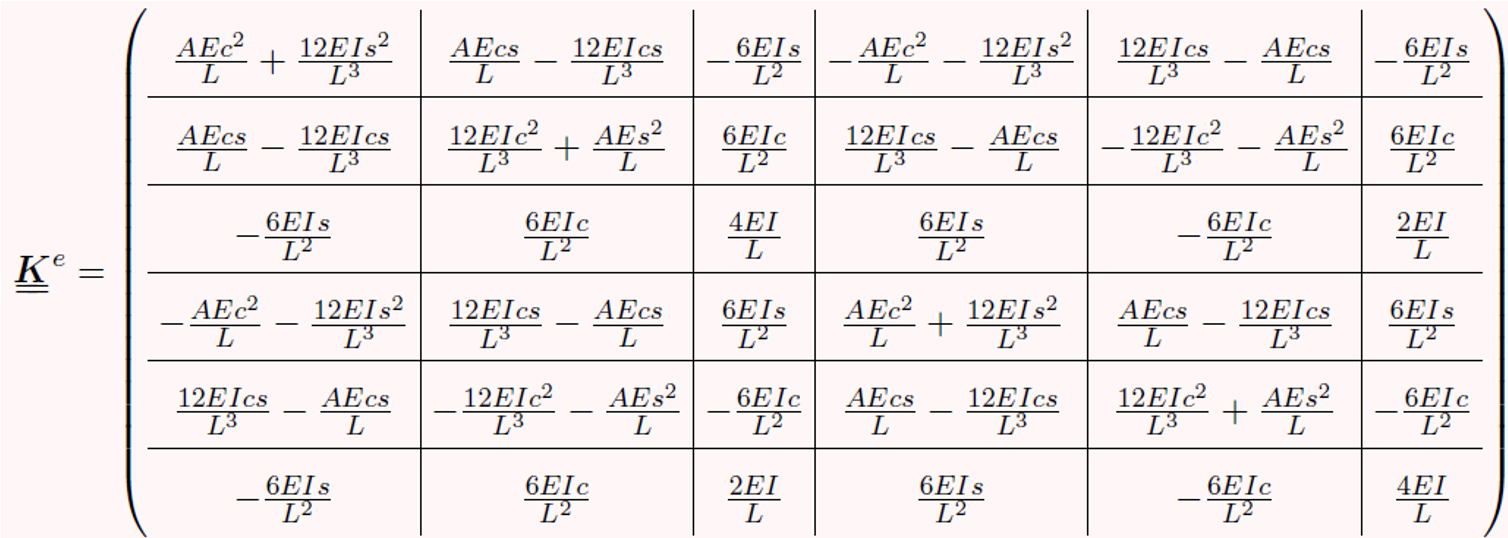
\includegraphics[width=\textwidth]{../Grafiken/globale_elementsteifigkeitsmatrix_zdb.png}
\end{frame}

\end{document}